\documentclass[11pt]{extarticle}
\usepackage{manualdoprofessor}
\usepackage{fichatecnica}
\usepackage{lipsum,media9}
\usepackage[justification=raggedright]{caption}
\usepackage[one]{bncc}
\usepackage[araucaria]{../edlab}
\usepackage{marginnote}
\usepackage{pdfpages}

\newcommand{\AutorLivro}{Edward Lear}
\newcommand{\TituloLivro}{Conversando com varejeiras azuis}
\newcommand{\Genero}{Conto; crônica; novela}
%\newcommand{\imagemCapa}{./images/PNLD2022-001-01.jpeg}
\newcommand{\issnppub}{XXX-XX-XXXXX-XX-X}
\newcommand{\issnepub}{XXX-XX-XXXXX-XX-X}
% \newcommand{\fichacatalografica}{PNLD0001-00.png}
\newcommand{\colaborador}{Renier Silva}

\begin{document}

\title{\TituloLivro}
\author{\AutorLivro}
\def\authornotes{\colaborador}

\date{}
\maketitle

\tableofcontents

\section{Carta ao professor}

Caros professores e professoras,

esperamos, com este material,
auxiliá-los no trabalho com o \textbf{Ensino Fundamental \textsc{ii}} em 
sala de aula. \textit{Conversando com varejeiras azuis}, de Edward Lear, é um livro singular
por vários motivos e possibilita atividades didáticas interessantíssimas,
como vocês acompanharão a seguir.

Começando com um conto que apresenta a aventura de crianças viajando 
ao redor do mundo à bordo de um barco, este livro proporcionará de fato
uma viagem da mesma magnetura aos jovens em sala de aula. 
Receitas de pratos inventados com ingredientes imaginados, 
plantas que dão peixes e pássaros, personagens impossíveis...
tudo tende ao lúdico. 

As atividades que aqui propomos têm como objetivo aproveitar
as sugestões feitas pelo próprio livro, desenvolvendo 
os aspectos que dizem respeito à criatividade na relação
com as linguagens e os conhecimentos científicos atrelados 
às situações que são apresentadas. 

Esperamos, professores, que este material sirva como um guia 
para seu trabalho em sala de aula. Já contamos, no entanto, com as adaptações
que surgirão organicamente na recepeção do mesmo por vocês, que possuem 
trajetórias e escolhas didáticas específicas, bem como no contato com os 
alunos, que tanto têm a oferecer para o enriquecimento da experiência didática.

Boa aula!


\section{Sobre o livro}

\textit{Conversando com varejeiras azuis} é um livro que reúne as principais
obras em verso, prosa e desenho de Edward Lear.
Ao todo, são 22 obras, algumas em prosa, outras em verso, divididas
em seis partes: 

\begin{itemize}
\item {``A história de quatro criancinhas que deram a volta ao mundo''} é
um conto sobre as aventuras \emph{nonsense} vividas por um grupo de crianças
que, sozinham, dão a volta ao mundo a bordo de um barco;
\item {``Culinária \emph{nonsense}''} como o próprio nome diz, 
são receitas de pratos e ingredientes inventados; 
\item {``Algumas espécies da botânica \emph{nonsense}''} seguindo a lógica das receitas inventadas,
aqui são seres vivos frutos de uma mistura entre elementos da natureza vegetal e da natureza
humana que são apresentados; 
\item {``Limeriques''} são poemas de quatro ou cinco versos acompanhados de ilustrações que contam
situações inusitadas e fantasiosas; 
\item {``O cinturão''} é um ``poema indiano'' feito durante a estadia do autor na Índia e conta a história de um 
monstro que engoliu donzelas indefesas; e, por fim,
\item {``O popular autor e viajante na Albanya e Calabrya, mantendo seus pês aquecidos''},
um divertido poema formado por enumeração e ilustração, com uma linguagem intencionalmente
estranha --- mantida na tradução para o português.
\end{itemize}


\reversemarginpar
\marginparwidth=5cm

%\marginnote{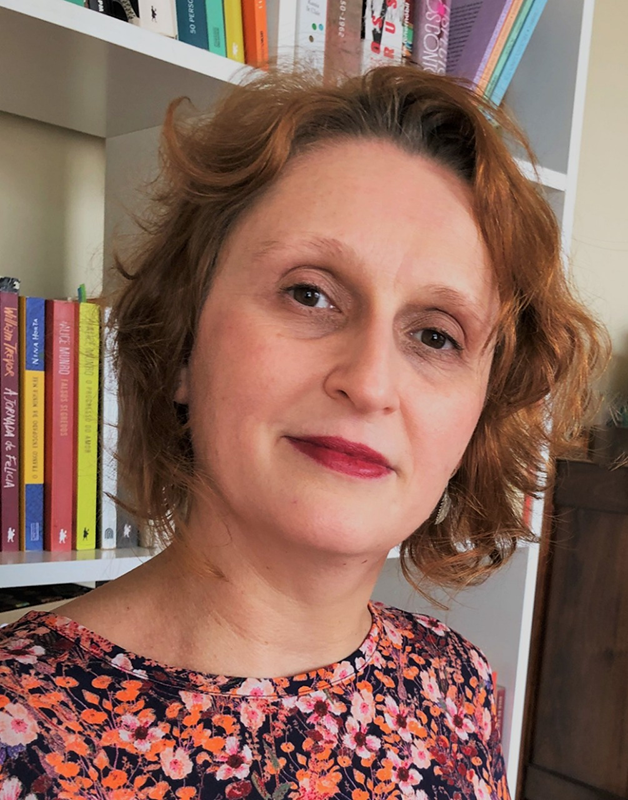
\includegraphics[width=\marginparwidth]{./images/PNLD2022-001-02.png}\\
%A autora Camila Werner (Arquivo pessoal)}


\section{Sobre o autor}

\Image{Edward Lear.(Domínio público)}{PNLD2023-032-01.jpg}

\paragraph{O autor} Desenhista, pintor, escritor e músico, Edward Lear nasceu em Londres, em
maio de 1812. É considerado, junto a Lewis Carrol, autor de \textit{Alice no país das maravilhas},
um dos criadores da literatura \textit{nonsense} da era vitoriana.
Ainda jovem, Lear deixou a Inglaterra devido a uma saúde debilitada:
sofria complicações respiratórias como asma e bronquite, além
de um quadro epiléptico que o acompanhou durante toda a vida.
Tais problemas desencadearam no autor ainda muito cedo,
por volta dos oito anos, sintomas depressivos. Lear sentia-se 
envergonhado perante a comunidade principalmente por conta das
crises de epilepsia. Seus pais logo decidiram, portanto,
que ele deveria viver numa região de clima mais ameno.

Essa mudança precoce e sua ida à Itália, aos 25 anos,
onde permaneceu por muito tempo, desenvolveram uma característica
que muito particular em sua personalidade: o sentimento de 
expatriado. Em sua cidade natal, Londres, ele era visto como um 
estrangeiro que só vê à cidade no verão; já em Roma, era um inglês, 
um turista qualquer que visitam a cidade no inverno. 

Edward Lear sempre fez questão, porém, de reafirmar sua identidade nacional:
era inglês. Na introdução do livro, Dirce do Amarante lembra que,
nas palavras de um estudioso, ainda que Lear pudesse ler e conviver com
os estrangeiros, ele não podia \textit{conversar} com eles.\footnote{\textsc{amarante}, 
Dirce Waltrick do. ``Volta ao mundo com Edward Lear'' in \textit{Conversando com varejeiras azuis} p.\,14.} 
Esta observação é fundalmental para se entender o olhar de Lear em sua 
produção artística. 

Próximo à Coroa britânica, chegando mesmo a ser professor particular
da Rainha Vitória à época da publicação de suas \textit{Excursões ilustradas na Itália}, de 1846,
Lear carregava consigo algo do olhar imperialista britânico, então no
auge de sua expansão. Viajou para muitos dos territórios do imperial,
com o intuito de buscar fontes de inspiração para suas ilustrações. 
De certo modo, a caricaturização e o ``sem sentido'' das personagens 
de sua obra podem ser um reflexo de sua incapacidade, herdada do projeto civilizatório 
do Império Britânico, de perceber os indivíduos locais em pé de igualdade. 

No entanto, essa relação é mais complexa do que se parece. Bem como seu próprio 
pertencimento à identidade britânica carrega ambiguidades, seu posicionamento 
também o faz. Dirce do Amarante diz que:

\begin{quote}

Na obra de Lear, a sociedade inglesa é representada pelo pronome ``eles''. E, ``eles'', 
como afirma o escritor Aldous Huxley, ``são 'a força da opinião pública''', que ``sem exceção, 
odeia excentricidades''.
Contudo, nos textos de Lear, não há uma defesa da sociedade repressora, tampouco do cidadão 
reprimido; o artista inglês apenas enfatiza a tensa relação e, às vezes, muito ocasionalmente, 
uma harmonia entre eles.\footnote{Ibidem. p.\,18.}

\end{quote}

Em sua lista de obras publicadas encontra-se \textit{Ilustrações da Família de Psittacidae, ou Papagaios}, de 1832,
\textit{Visões em Roma e seus arredores}, de 1841, \textit{Um livro de \emph{nonsense}}, de 1846,
\textit{Excusões ilustradas na Itália}, de 1846, \textit{Tortoises, Terrapins and Turtles}, de 1872,
\textit{Laughable Lyrics}, de 1877, \textit{Botânica \emph{nonsense}}, 1888, entre outros.



\paragraph{A literatura \textit{nonsense}} É provavelmente do livro de Edward Lear intitulado
\textit{Um livro de \emph{nonsense}}\footnote{\textit{A book of \emph{nonsense}}, no original.},
de 1846, que tenha se originado o então estabelecido termo \textit{nonsense} na literatura. 

De modo geral, a literatura \textit{nonsense} se caracteriza por uma recusa
às normas da lógica e da razão, presente inclusive na linguagem, 
e uma abertura à criatividade na forma de exergar o mundo e de 
escrever. 

\begin{quote}
O vezo da significação, da evocação e elaboração de sentido já está por demais arraigado na
linguagem. O que se tenta fazer \textit{nonsense} é driblar o sentido, por meio da
justaposição de sentidos parciais e opostos, do solapamento e
embaralhamento das várias camadas comunicativas. Não se podendo evitar
a criação de sentido, tenta-se evitar seu assentamento a todo custo.\footnote{\textsc{ávila}, M. \textit{Rimas e Solução.}
p.\,115--116.}
\end{quote}

\Image{Ilustração presente no \textit{livro de \emph{nonsense} de Edward Lear. (CC BY 2.0).}}{PNLD2023-032-02.jpg}

As personagens da literatura \textit{nonsense} possuem a característica
de serem extremamente solitárias. Via de regra, são indivíduos que se encontram
frente a todo um grupo. Mas essa solidão não é expressa de modo lírico ou romântico.
Ela não leva o leitor à comoção. O \textit{nonsense} não precisa do emocionalismo. 
A natureza dessa solidão é a incomunicação, ou seja, a solidão se dá pela incapacidade
da linguagem de estabelecer ou promover comunicação

Por fim, o \textit{nonsense} é criado por uma linguagem que modifica a realidade.
Ou seja, a linguagem precede a realidade, criando as regras segundo as quais
esta vai funcionar. 

\paragraph{Uma época de contradições}

A Era Vitoriana compreende o período em que a rainha Alexandrina Victoria (1819--1901)
esteve no trono do Reino Unido da Grã-Bretanha.
Trata-se de uma época, no mínimo, contraditória. Por um lado, testemunhou-se o
assentamento do Império Britânico e o auge da Revolução Industrial; por outro, produziu-se 
uma verdadeira legião de miseráveis, explorada como mão de obra barata, que vivia amontoada 
em moradias de péssima qualidade, tornando-se alvo de doenças infecciosas e epidemias derivadas da 
falta de higiene e da população excessiva

Mesmo entre as classes abastadas, o paradoxo existiu, pois, sob a aparência de um arraigado
apego à moral e à religião, havia uma clandestinidade em que a depravação, a luxúria
e o espiritualismo eram comuns.

O estilo de vida modelar vitoriano assumiu um caráter controlador.
Como diz Foucault na \textit{Microfísica do poder}, os corpos passaram a ser disciplinados e vigiados, 
o que, na realidade, não impedia a transgressão das normas, pois os
austeros chefes das famílias rendiam-se ao afloramento do desejo pelo proibido, frequentando
bordeis secretamente. As prostitutas, geralmente vistas como anomalias, contraditoriamente,
eram consideradas uma contrapartida indispensável à solidez familiar, uma vez que, ao
entregarem-se a prazeres proibidos, dando vazão à sensualidade, os homens se tornavam mais
aptos a exercer o papel social de esposos e pais. 

\section{Sobre o gênero}

\paragraph{O gênero} O gênero deste livro é a \textit{conto; crônica; novela}. 

%596 caracteres
\paragraph{Descrição} O que define um gênero narrativo é o fato de, não importa
qual seja sua forma, eles \textit{contarem uma história}.
As especificidades do \textit{como} esta história será contada é que
qualificaram os tipos de gênero narrativo, que podem ser: conto, crônica, novela,
epopeia, romance ou fábula. 

Toda narrativa possui, necessariamente, um narrador, uma personagem, um enredo,
um tempo e um espaço. O narrador, ou narradora, pode ser onisciente, literalmente
\textit{que tudo sabe}, observador ou personagem --- categorias que não são autoexclusivas.
O discurso elaborado por este narrador ou narradora pode ser direto, indireto ou indireto livre 
--- ou seja, ele ou ela pode aparecer mais diretamente ou mais indiretamente; no último caso,
sua voz se mistura à das personagens da história.

O narrador \textbf{não é necessariamente} a voz do autor. É errada a afirmação
de que o autor fala através do narrador de uma história. É bastante comum,
há algum tempo na história literária, sobretudo desde os pré-modernistas, que 
o narrador represente justamente o contrário do que pensa o autor. Neste caso, 
utiliza-se elementos como a \textbf{ironia} para sugerir que o autor \textit{não é confiável}.

Já as persponagens variam quanto a sua \textbf{profundidade}. Há personagens planas, ou
personagens-tipo, e personagens redondas, ou complexas. Personagens planas
são facilmente repetíveis pois se amparam em lugares-comuns da cultura, como
o vilão, o herói, a vítima, o palhaço, tudo isso com marcações de gênero e espécie ---
o herói tradicionalmente é um homem, a vítima, uma mulher, e o vilão, uma figura que 
se afasta da humanidade por alguma razão, às vezes sobrenatural. 
Personagens redondos, por outro lado, estão mais próximos das \textit{pessoas reais}.
Uma personagem complexa pode ser, em um dado momento da narrativa, vilã, e em 
outro, heroina. É importante notar como as visões de mundo, um traço cultural e 
portanto relativo, influenciam na caracterização das personagens, planas 
ou redondas, de uma história.

O tempo de uma narrativa pode ser cronológico ou psicológico.
No tempo cronológico, o enredo segue a ordem ``normal'' dos acontecimentos,
aquela marcada pelo relógio e pelo calendário. Os acontecimentos vêm um após o 
outro e se delimita muito bem \textit{passado}, \textit{presente} e \textit{futuro}.
Já no tempo psicológico, segue-se uma ordem \textit{subjetiva} dos acontecimentos, 
e portanto, \textit{não linear}, já que a influência emocional e psíquica 
da subjetividade afeta a racionalidade do tempo cronológico. 

O espaço, por fim, é o lugar onde se passa a narrativa. Dependendo do caso, 
ele pode funcionar mais como um plano de fundo, sem muita interferência
no enredo, ou mais ativamente, aproximando-se das características das personagens
e influenciando no desenrolar da trama. 

O último aspecto de um gênero narrativo que podemos abordar é sua 
\textit{extensão}. Dentre os elementos que distinguem um subgênero 
de outro é o tamanho da história: uma crônica e um conto são \textit{necessariamente}
curtos, ao passo que uma epopeia e um romance, são longos. Uma novela
está no ponto intermediário entre um romance e um conto.
Ainda poderíamos falar dos registros de cada subgênero: 
a epopeia é originalmente um subgênero \textit{oral}, versificado, e metrificado,
já o romance é tradicionalmente \textit{escrito} em prosa. 
Desde meados do século \textsc{xviii}, no entanto, o estabelecimento
dos gêneros e subgêneros narrativos tornam-se cada vez menos rígido,
com as características cada vez mais fluidas e intercomunicativas.

Como o presente livro se trata de uma narrativa \textit{curta},
finalizamos com as palavras de Luiza Vilma Pires a respeito do
subgênero:

\begin{quote}
sob o nome de narrativa curta, estão situadas obras que apresentam uma trama 
um pouco mais complexa, que ocorre em diversos espaços e em uma temporalidade 
que pode ser de vários dias, semanas ou meses. Entretanto a função das ilustrações 
continua as mesmas, são complementares à história e contribuem para sua compreensão. 
Os temas relacionam-se a vivência infantis (brincadeiras, passeios, pequenas aventuras), 
a aspectos ligados à interioridade das personagens (busca de identidade, insegurança, 
medos) ou a relações interpessoais (desentendimentos familiares, entre amigos, solidariedade).\footnote{“Narrativas infantis”, de Luiza Vilma Pires Vale. In \textsc{saraiva}, J. A. (Org.) \textit{Literatura e alfabetização: do plano do choro ao plano da ação}. Porto Alegre: Artmed, 2001.} 
\end{quote}

\section{Atividades}

\subsection{Pré-leitura}

\subsubsection{Atividade 1}

\BNCC{EF35EF01}
\BNCC{EF35EF01}
\BNCC{EF15AR09}

\paragraph{Tema} Brincando com o lúdico.

\paragraph{Conteúdo} Introduzir os alunos e alunas ao trabalho com o 
universo lúdico a partir de brincadeiras de seu quotidiano ou não.

\paragraph{Justificativa} A literatura \emph{nonsense} presente na obra 
do escritor Edward Lear se caracteriza por uma abordagem subversiva da realidade. 
Para tanto, o autor cria suas próprias regras para criar suas histórias,
poemas, objetos e seres vivos. O \emph{nonsense}, bem como o universo lúdico,
estão ligados à área da criatividade, e por isso, os alunos e alunos
devem estar inseridos neste contexto para ter uma boa aproximação da
obra que lerão nas aulas seguintes.  

\paragraph{Metodologia} Propomos como brincadeira inicial a \textbf{mímica}.
Num espaço apropriado, que pode ser a própria sala de aula com as cadeiras
afastadas, o aluno ou aluna deve ir ao centro e imitar por meio de gestos 
o elemento que tem em mente. É interessante que se estabeleça à 
priori alguma categoria  para que a brincadeira seja realizável, como
por exemplo: animais, profissões etc.

Outra brincadeira que pode ser interessante neste contexto 
é o \textbf{cadáver esquisito}. Originado no começo do século \textsc{xx} na França
sob a influência do movimento surrealista, trata-se da construção de uma história a partir
de frases aleatórias.

Separe uma folha de papel. Mostre diferentes imagens que podem ser
obras de artes, pinturas, fotografias etc. Cada aluno ou aluna
deve escrever uma frase a partir do que vê na mesma folha.
O mais importante é: cada vez que uma frase for escrita, o papel deve ser
dobrado, de modo que o aluno ou aluna seguinte não veja o que foi escrito.
Quando todos tiverem escrito sua frase, abra o papel e leia a história. 

\paragraph{Tempo estimado} Duas aulas de cinquenta minutos.


\subsection{Leitura}

\BNCC{EF04LP25}

\subsubsection{Atividade 1}

\paragraph{Tema} Virando um chef de culinária \emph{nonsense}.

\paragraph{Conteúdo} Criar pequenas esquetes de teatro a partir das receitas de culinária \emph{nonsense}.

\paragraph{Justificativa} Esta atividade deverá trabalhar competências que dizem respeito, primeiro,
à adaptação de um texto não dramático a um texto dramático, e depois, à experiência de encenação cênica. 
Deste modo, tanto competências linguísticas, sociocomunicativas e artísticas serão mobilizadas neste trabalho. 

\paragraph{Metodologia} No primeiro momento, o professor ou professora deve fazer uma leitura oral
e conjunta com os alunos e alunos das três receitas da seção ``Culinária \emph{nonsense}'' do livro. 

Depois, separados em grupos, eles devem trabalhar os textos para apresentá-los 
como se fossem um chef de cozinha ensinando a fazer uma receita. 
Você pode perguntar se eles conhecem algum chef de cozinha, 
se assistem algum programa de culinária na televisão ou na Internet. 
Caso alguém não tenha referência do assunto, mostre um vídeo 
de um chef ensinando a fazer uma receita. 

Detalhes da encenação teatral devem ser pensados tais como \textbf{cenário},
\textbf{figurino} e \textbf{caracterização}. 

\begin{itemize}
	\item Como se chama este ou esta chef?
	\item Onde ele ou ela nasceu?
	\item Como ele ou ela se veste?
	\item Ele ou ela tem sotaque? 
\end{itemize}

Além disso, deve se dar uma importância especial ao \textbf{texto} que deve
ser \textbf{decorado}. 

Para esta importante e desafiadora etapa, dê algumas dicas aos alunos
que podem estar experimentando-a pela primeira vez:

\begin{itemize}
	\item Ler o texto em voz alta;
	\item Escrevê-lo à mão;
	\item Ler e fazer um resumo com as próprias palavras;
	\item Pedir para alguém ler o texto para você;
	\item Gravar o texto e escutá-lo;
	\item Interagir com o texto por meio de gestos e expressões corporais;
	\item Fazer pausas durante a leitura.
\end{itemize}

\paragraph{Tempo estimado} Duas aulas de cinquenta minutos.

\subsubsection{Atividade 2}

\BNCC{EF04GE09}

\paragraph{Tema} Cartografia \emph{nonsense}.

\paragraph{Conteúdo} A partir do conto ``A história de quatro criancinhas que deram a volta ao mundo'',
criar um mapa onde se representem os lugares por onde passam as personagens da história.

\paragraph{Justificativa} A cartografia é um instrumento da área da Geografia utilizado para 
criar mapas. Um mapa é uma representação gráfica e métrica de uma porção de território sobre 
uma superfície bidimensional, geralmente plana, embora também possa ser esférica como é o caso 
dos globos terrestres. Grosso modo, um mapa é uma leitura de uma região: uma cidade, um país, 
ou uma rota. À época da Idade Média e com o começo das Grandes Navegações, época de desenvolvimente
da cartografia, era comum a presença de monstros marinhos em mapas tanto do mundo quanto de partes da Europa.

\Image{Mapa da Islândia de 1609 feito Abraham Ortelius. (CC BY 2.0)}{PNLD2023-032-03.jpg}

Será importante para os alunos e alunas perceberem como, ainda que o \emph{nonsense} seja
por definição um afastamento da realidade, nesta mesma realidade existem, em diferentes momentos
da História, elementos que poderíamos chamar de fantasiosos. Desenhar um mapa, portanto, 
é antes de tudo uma atividade de criação que pode servir a fins diversos, mais
científicos ou mais artísticos --- ainda que um não negue o outro necessariamente.

\paragraph{Metodologia} A partir do exemplo do mapa da Islândia e de outros que o professor
ou professora pode facilmente encontrar na Internet, peça aos alunos que criem
uma representação cartográfica do conto que acabaram de ler. 
Eles podem se inspirar nas ilustrações de Edward Lear para desenhar as criaturas. 

\Image{Uma das criaturas ilustradas no conto de Edward Lear. (Retirado do livro).}{PNLD2023-032-05.jpg}

Ao fim da aula, todos devem apresentar o resultado do trabalho.
Faça-os perceber como \textbf{a mesma referência, o conto que todos leram,
pode dar origem a uma diversidade de produções --- todas interessantes}.


\paragraph{Tempo estimado} Duas aulas de cinquenta minutos.


\subsection{Pós-leitura}

\subsubsection{Atividade 1}

\paragraph{Tema} Criação de uma história \emph{nonsense}.

\paragraph{Conteúdo} Elaborar individualmente uma história, seja em prosa ou
em versos, onde o \emph{nonsense} seja o fio condutor. 

\paragraph{Justificativa} Após todas as atividades de sensibilização 
em relação ao lúdico e às possibilidades de criação por meio da linguagem, 
os alunos e alunas devem se apropriar desta técnica.
Para isso, nada mais apropriado do que uma oficina de criação literária. 

\Image{``Pé de peixes'', uma das espécies da botânica \emph{nonsense}. (Retirado do livro).}{PNLD2023-032-04.jpg}

\paragraph{Metodologia} O ponto de partida pode vir de diversos lugares.
Pode ser feita uma nova rodada do jogo \textbf{cadáver esquisito},
por exemplo. Outra possibilidade, é se começar a partir de um estímulo
visual, que pode ser inlcusive as próprias ilustrações de Edward Lear 
no livro. 

Os alunos e alunas devem ser estimulados a não só escrever mas também a 
ilustrar suas histórias. Conforme a relação com o texto, eles e elas
devem criar suas próprias regras para a elaboração dos desenhos. 
Não precisam nem devem se preocupar em parecer realistas, 
mas antes, colocar a significação em risco --- uma planta que,
como frutos, dá  peixes, ou pássaros, por exemplos. 

Ao fim da atividade, os trabalhos serão apresentados numa roda de contação de histórias. 

\paragraph{Tempo estimado} Quatro aulas de cinquenta minutos.


\subsubsection{Atividade 2}

\BNCC{EF15AR24}
\BNCC{EF03LP13}

\paragraph{Tema} Oficina de contação de histórias. 

\paragraph{Conteúdo} Organização de uma roda de contação de histórias
com protagonismo dos alunos e alunas.

\paragraph{Justificativa} Dando continuidade à atividade de teatralização das
receitas na atividade de leitura, a contação de histórias trabalha competências
que dizem respeito ao campo linguístico e sociocomunicativo. 
Ao contar uma história, o indivíduo se apropria do lugar do narrador e
atuar como cocriador da mesma. Além do conteúdo propriamente dito 
da história, toda a estrutura linguística e gramatical, a sintaxe 
e o vocabulário presentes no texto serão trabalhados. 
O grande diferencial desta atividade é que seu objetivo não está 
exclusivamente no exercícios destas capacidades linguísticas, 
mas sim ligados a elas e à capacidade de \textbf{apresentar oralmente}
um texto a um público. Fala e corpo estão totalmente ligados nesta atividade. 

\paragraph{Metodologia} Divida a turma em grupos que serão 
responsáveis pela organização da roda de contação de histórias. 


\paragraph{Tempo estimado} Duas aulas de cinquenta minutos.


\section{Sugestões de referências complementares}

\paragraph{Músicas e víeos}

\begin{itemize}
\item ``Mafagafolândia''. Cia Mafagafos. Disponível em \url{https://www.youtube.com/watch?v=MYZm-aR2IJU}. Último acesso em 24 de dezembro de 2021.


\item ``Fabulário cantado''. Cia Mafagafos. Disponível em \url{https://www.youtube.com/watch?v=0tWcd7Xvbbs}. último acesso em 24 de dezembro de 2021.

O espetáculo de narração oral cênica, teatro de animação e música. ``Fabulário Cantado'' foi concebido pela Cia Mafagafos baseado em fábulas de Esopo, Fedro e La Fontaine.  As histórias e músicas são narradas e executadas com o uso de bonecos, objetos e adereços, além de instrumentos musicais. 


\end{itemize}


\paragraph{Livros e artigos}

\begin{itemize}
	
\item \textsc{diegues júnior}, Daniel. \textit{Literatura popular em verso}. Estudos. Belo Horizonte: Itatiaia, 1986. 

\item \textsc{marco}, Haurélio. \textit{Breve história da literatura de cordel}. São Paulo: Claridade, 2010.

\item \textsc{nuvens}, Plácido Cidade. \textit{Patativa e o universo fascinante
do sertão}. Fortaleza: Fundação Edson Queiroz, 1995.

\item \textsc{tavares}, Braulio. \textit{Contando histórias em versos. Poesia e romanceiro popular no Brasil}. São Paulo: 34, 2005.

\item \textsc{tavares}, Braulio. \textit{Os martelos de trupizupe}. Natal: Edições Engenho de Arte, 2004.
\end{itemize}

\section{Bibliografia comentada}

\subsection{Livros}

\begin{itemize}

	\item \textsc{albrecht}, Tatiana D'Ornellas. \textit{Atividades lúdicas no Ensino Fundamental}. Universidade Católica Dom Bosco, \textsc{ms}, 2009. Disponível em: \url{https://site.ucdb.br/public/md-dissertacoes/8072-atividades-ludicas-no-ensino-fundamental-uma-intervencao-pedagogica.pdf}. Último acesso em 24 de dezembro de 2021.

	As atividades lúdicas, quando bem aplicadas e no momento oportuno, trazem
grandes benefícios. Contudo, a grande maioria das escolas não utiliza esse instrumento. Por
que será que existe essa resistência por parte das escolas e dos professores? Por que não
adequar o lúdico ao cotidiano escolar de maneira prática, educativa e ao mesmo tempo
divertida?

\item \textsc{brasil}. Ministério da Educação. Base Nacional Comum Curricular. Brasília, 2018.

Consultar a \textsc{bncc} é essencial para criar atividades para a turma. Além de especificar 
quais habilidades precisam ser desenvolvidas em cada ano, é fonte de informações sobre 
o processo de aprendizagem infantil. 

 \item \textsc{bandoch}, Adriana Rodrigues Vieira. \textit{A inserção do teatro nas séries iniciais do Ensino Fundamental}.
 Universidade Tecnológica Federal do Paraná, 2012. Disponível em: \url{http://repositorio.utfpr.edu.br/jspui/bitstream/1/20738/2/MD_EDUMTE_II_2012_03.pdf}. Último acesso em 24 de dezembro de 2021.

	O teatro no Ensino Fundamental é uma das formas de se trabalhar o conhecimento,
pois nele há a possibilidade do ser humano em se integrar, vivenciar, expressar e
criar situações, condições para novas aprendizagens éticas, sociais, culturais,
históricas.


\item \textsc{van der linden}, Sophie. Para ler o livro ilustrado. São Paulo: Cosac Naify, 2011.

Livro sobre as particularidades do livro ilustrado, que apresenta as diferenças entre o livro ilustrado e o livro com ilustração. 
\end{itemize}

\subsection{Vídeos}

\begin{itemize}

\item {\textsc{amarante}, Dirce Waltrick do. \textit{Literatura \emph{nonsense} para crianças: Edward Lear e
Gertrude Stein}.} Disponível em: \url{https://www.youtube.com/watch?v=2hhvZFCfLlg}. Último acesso de 24 de dezembro de 2021. 

Fala da organizadora e tradutora do livro \textit{Conversando com varejeiras azuis}, Dirce Waltrick do Amaral,
em série de encontros acerca da Literatura Infantil. Neste encontro, o tema é a Literatura \emph{nonsense},
onde a autora trata dos trabalhos de Edward Lear e Gertrude Stein.

\end{itemize}

\end{document}